\documentclass{ctexart}
% 数学公式
\usepackage{amsmath, amssymb, mathtools}
%处理图片
\usepackage{graphicx}
\usepackage{float}
\usepackage{subfigure}
% 序号
\usepackage{enumerate}
% 页面设置
\pagestyle{plain}
\usepackage[a4paper, top=1in, bottom=1in, left=1.5in, right=1.5in]{geometry}
\usepackage[fontsize=12]{fontsize}
% 文档内容
\begin{document}

\title{稳态误差}
\author{ecstayalive}
\maketitle

\section*{理解稳态误差}

在讨论这个问题是,我们必须遵循如下的前提:即稳态误差相关问题只有当系统稳定时才具有意义。
这一点显而易见,不再讨论。同时关于稳态误差篇幅不多,主要在于理解。

\subsection*{两种定义,what are they?}

我们经常会看到两种定义的稳态误差,一种是输入端定义的稳态误差,一种是输出端定义的稳态误差。

先让我们讨论一下稳态误差的第一种定义,这种定义的稳态误差在图中位置如下图:

%H为当前位置,!htb为忽略美学标准,htbp为浮动图形
\begin{figure}[H]
    %图片居中
    \centering
    %插入图片,[]中设置图片大小,{}中是图片文件名
    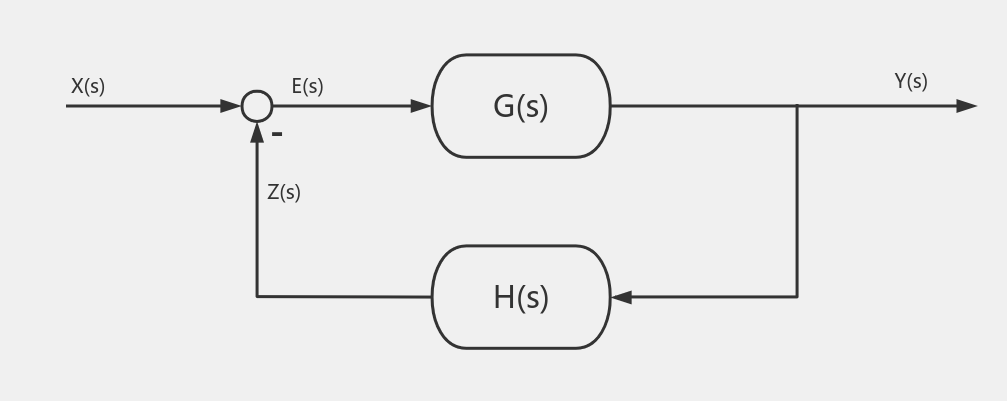
\includegraphics[width=0.8\textwidth]{./pics/steady_state_error/control_system.png}
    %最终文档中希望显示的图片标题
    \caption{输入端误差函数定义}
    %用于文内引用的标签
    \label{Fig.1}
\end{figure}

图\ref{Fig.1}中的$E(s)$即是误差的Laplace变换。此时,我们也可以写出来输入端误差的数学表达
式:
\begin{equation}
    \begin{aligned}
        E(s) & = X(s) - Z(s)      \\
             & = X(s) - H(s) Y(s)
    \end{aligned}
\end{equation}

这便是输入端定义地稳态误差,还有另外一种定义,即输出端定义,此时其数学表达式为如下,即输入
的Laplace变换直接减去输出的Laplace变换:
\begin{equation}
    \begin{aligned}
        E(s) & = X(s) - Y(s)
    \end{aligned}
\end{equation}
我们现在已经知道了两种定义的形式,那为什么要这两种定义的形式呢?

因为对于输入端定义而言,我们在构建电路时是可以直接测量得到,便于输出,但是这种方式并不直观。
因为我们的输入往往和输出是统一单位。就比如,在构建一个运动系统是,我们希望电机移动$1^\circ$
,那么自然而然我们希望这个系统的输出就是电机移动了多少度。因此输出端定义的误差函数更加直观,
但是却难以直接测量。并且值的注意的是,\textbf{在单位负反馈的情况下,这两种定义的方式
    是一样的。}

但是除此之外,还有另外一种情况,就是题目本身定义了一个$E(s)$。这时候我们得额外的注意,
因为我们所作的任何操作不能影响$E(s)$在题目中的位置,否则就有可能出现错误。

\subsection*{稳态误差系数法}
首先我们应该记住,最基本的求解稳态误差的方法就是遵循如下的流程求出$\frac{E(s)}{X(s)}$:
\begin{enumerate}
    \item 判稳;
    \item 判定系统的稳态误差定义,是输出端定义还是输入端定义或者是题目自身给定的定义;
    \item 求出$\frac{E(s)}{X(s)}$;
    \item 确定输入函数$X(s)$;
    \item 使用终值定理求解$e_{ss}$;
\end{enumerate}

只不过,这种方法有时候太过繁琐,所以我们使用稳态误差系数方法。\textbf{但是,千万注意,稳态误差系数法
    是有一些使用条件的,如果这些条件不符合或者本身符合,但是却让人难以判断,令人困扰。那就不要使用
    这个方法,去使用上述的最基本的方法。}

现在我们假定你们已经知道了如何求解$K_p$、$K_v$与$K_a$的值。

那么我们先从单位负反馈系统开始讨论。这个结论十分简单,由于此时系统的误差的输入端的定义与
输出端的定义是完全一样的,我们只需要求出$G(s)$,然后直接计算就可以了。

那么当系统不是单位负反馈的情况呢?这时候如果系统定义的输入端的定义,那么我们已经知道
误差必然符合如下的公式:
\begin{equation}
    \frac{E(s)}{X(s)} = \frac{1}{1 + G(s)H(s)}
\end{equation}
那么此时我们可以毫无顾虑的使用稳态误差系数法。

但是如果系统稳态误差为输出端的定义,情况就变的不一样了。即系统框图如下:
%H为当前位置,!htb为忽略美学标准,htbp为浮动图形
\begin{figure}[H]
    %图片居中
    \centering
    %插入图片,[]中设置图片大小,{}中是图片文件名
    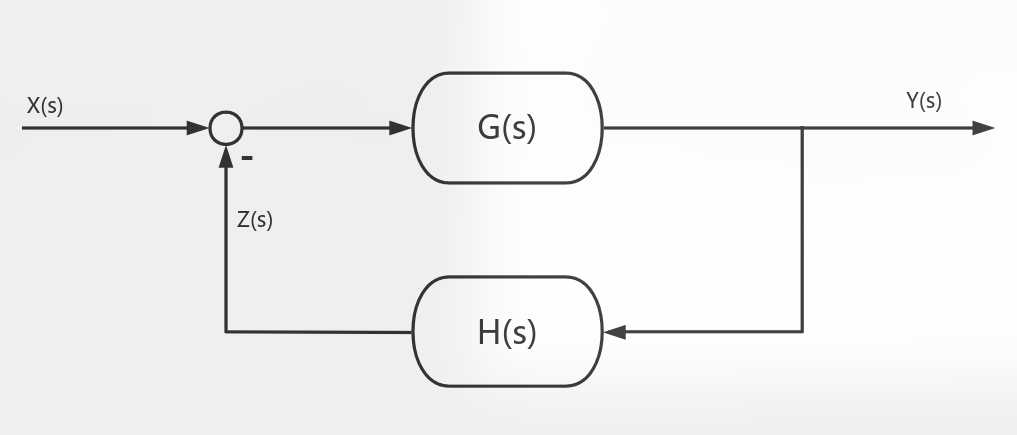
\includegraphics[width=0.8\textwidth]{./pics/steady_state_error/sys1.png}
    %最终文档中希望显示的图片标题
    \caption{系统框图}
    %用于文内引用的标签
    \label{Fig.2}
\end{figure}
并且误差有如下的定义:
\begin{equation}
    E(s) = X(s) - Y(s)
\end{equation}

那么我们可以计算出来:
\begin{gather}
    E(s) = X(s) - Y(s) \\
    E(s) = X(s) - \frac{G(s)}{1 + G(s)H(s)} X(s) \\
    E(s) = \frac{1 + G(s)H(s) - G(s)}{1 + G(s)H(s)} X(s)
\end{gather}

你就会发现,这个$E(s)$与上述的表达式相差甚远,当然也就无法使用稳态误差系数法了。
可是,我们十分希望使用这种方法,因为实在是太简单了,怎么办呢?我们发现在输出端定义
中,只是单纯的$X(s) - Y(s)$。而同时$Y(s)$却至于$X(s)$与$\Phi(s)$有关。
这也就是说,我只需要让系统闭环传函$\Phi(s)$保持不变,我当然可以将这个系统变为单位负反馈
系统,进而使得我们能够使用稳态误差系数法求解系统的稳态误差。下图便是我们等效的单位负反馈
系统框图。
%H为当前位置,!htb为忽略美学标准,htbp为浮动图形
\begin{figure}[H]
    %图片居中
    \centering
    %插入图片,[]中设置图片大小,{}中是图片文件名
    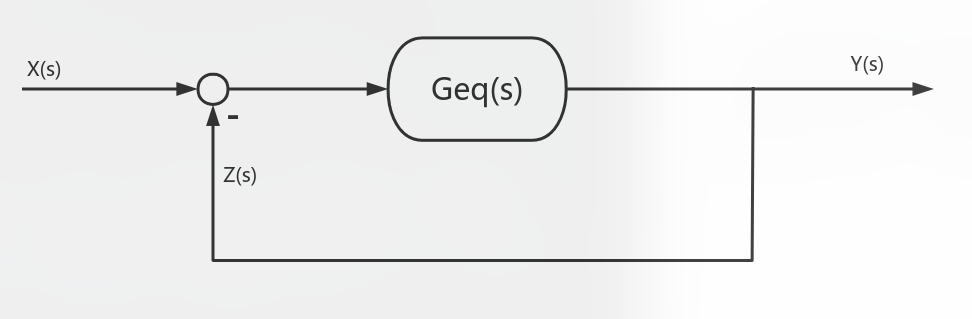
\includegraphics[width=0.8\textwidth]{./pics/steady_state_error/eq_sys.png}
    %最终文档中希望显示的图片标题
    \caption{等效系统框图}
    %用于文内引用的标签
    \label{Fig.3}
\end{figure}

这时我们可以得到如下的公式
\begin{equation}
    \begin{aligned}
        \Phi(s) = \frac{G(s)}{1 + G(s)H(s)} = \frac{G_{eq}(s)}{1 + G_{eq}(s)} = \frac{N(s)}{D(s)}
    \end{aligned}
\end{equation}

于是我们便可以得到:
\begin{equation}
    G_{eq}(s) = \frac{N(s)}{D(s) - N(s)}
\end{equation}

使用这个公式,我们便可以对非单位负反馈系统下输出端定义的稳态误差使用稳态误差系数法。

所以我们有如下的结论,或者是流程:
\begin{enumerate}
    \item 先看题目中的稳态误差的定义,是输入端定义,还是输出端定义,还是题目自己定义的随便一个。
    \item 如果是输入端定义或者是输出端定义的稳态误差
          \begin{enumerate}
              \item 看系统是不是单位负反馈系统,如果是,直接使用稳态误差系数法。
              \item 如果不是,输入端定义的话,找到$G(s)H(s)$后,使用该方法,输出端定义的话,求出$G_{eq}(s)$后使用该方法。
          \end{enumerate}
    \item 如果是系统定义的稳态误差,那么除非你较为容易的看出应该作出和中变换,并且这个变换不能改变定义的$E(s)$的位置,否则就别使用稳态误差系数法,就直接计算$\frac{E(s)}{X(s)}$
\end{enumerate}

说到这里,可能会有点迷,下面让我们看几道题目。

\subsection*{一些例题}
\subsubsection*{例题1}
%H为当前位置,!htb为忽略美学标准,htbp为浮动图形
\begin{figure}[H]
    %图片居中
    \centering
    %插入图片,[]中设置图片大小,{}中是图片文件名
    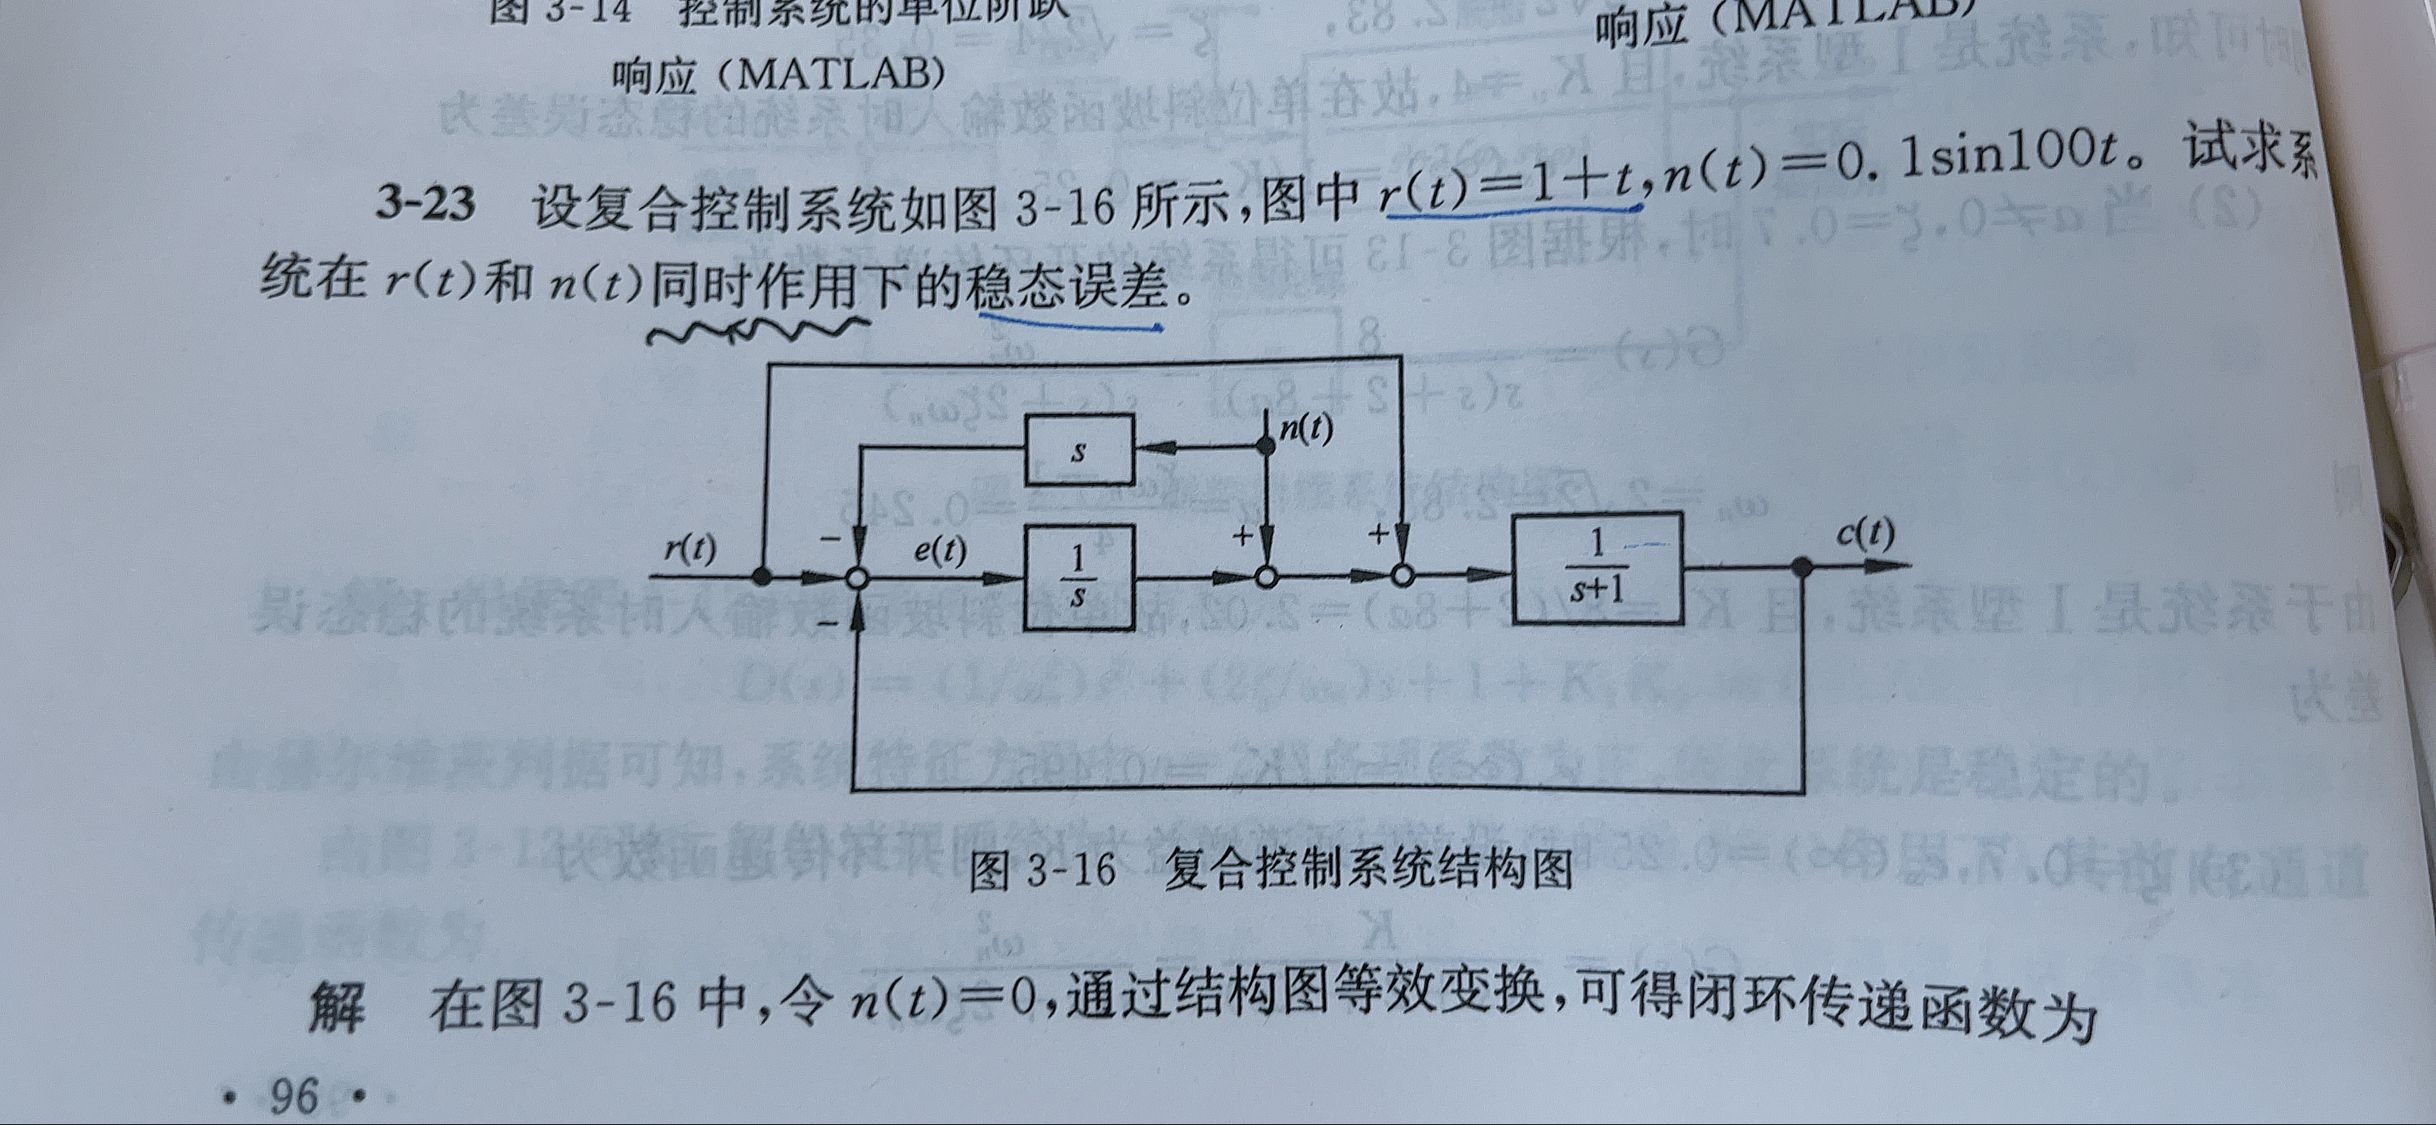
\includegraphics[width=0.9\textwidth]{./pics/steady_state_error/example1.jpg}
    %最终文档中希望显示的图片标题
    \caption{例题1}
    %用于文内引用的标签
    \label{Fig.4}
\end{figure}

按照流程,先来看一下$e(t)$是那种定义,是输入端定义吗?不是,因为前面有一个前馈,是输出端定义
吗?也不是,并且我们没能一眼看出能够作出的让$e(t)$不动的变换。因此,此时最稳妥的办法就是写
处$\frac{E(s)}{X(s)}$。对于这道题,在$N(s)=0$时,我们能够写出:
\begin{gather}
    E(s) = R(s) - E(s)\frac{1}{s(s+1)} - R(s)\frac{1}{s+1} \\
    E(s) = \frac{s^2}{s^2 + s + 1}R(s)
\end{gather}

这时给定$R(s)$就可以求出$e_{ss}$。当然如果对于稳态误差系数法有某些喜爱的话,
我们知道使用稳态误差系数的前提是$E(s)$可以写成:
\begin{equation}
    E(s) = \frac{1}{1 + G_{eq}(s)} R(s)
\end{equation}

这是你利用两个式子相等就可以求出$G_{eq}(s)$。但是并不建议这样做。因为完全多此一举。

\subsubsection*{例题2}
%H为当前位置,!htb为忽略美学标准,htbp为浮动图形
\begin{figure}[H]
    %图片居中
    \centering
    %插入图片,[]中设置图片大小,{}中是图片文件名
    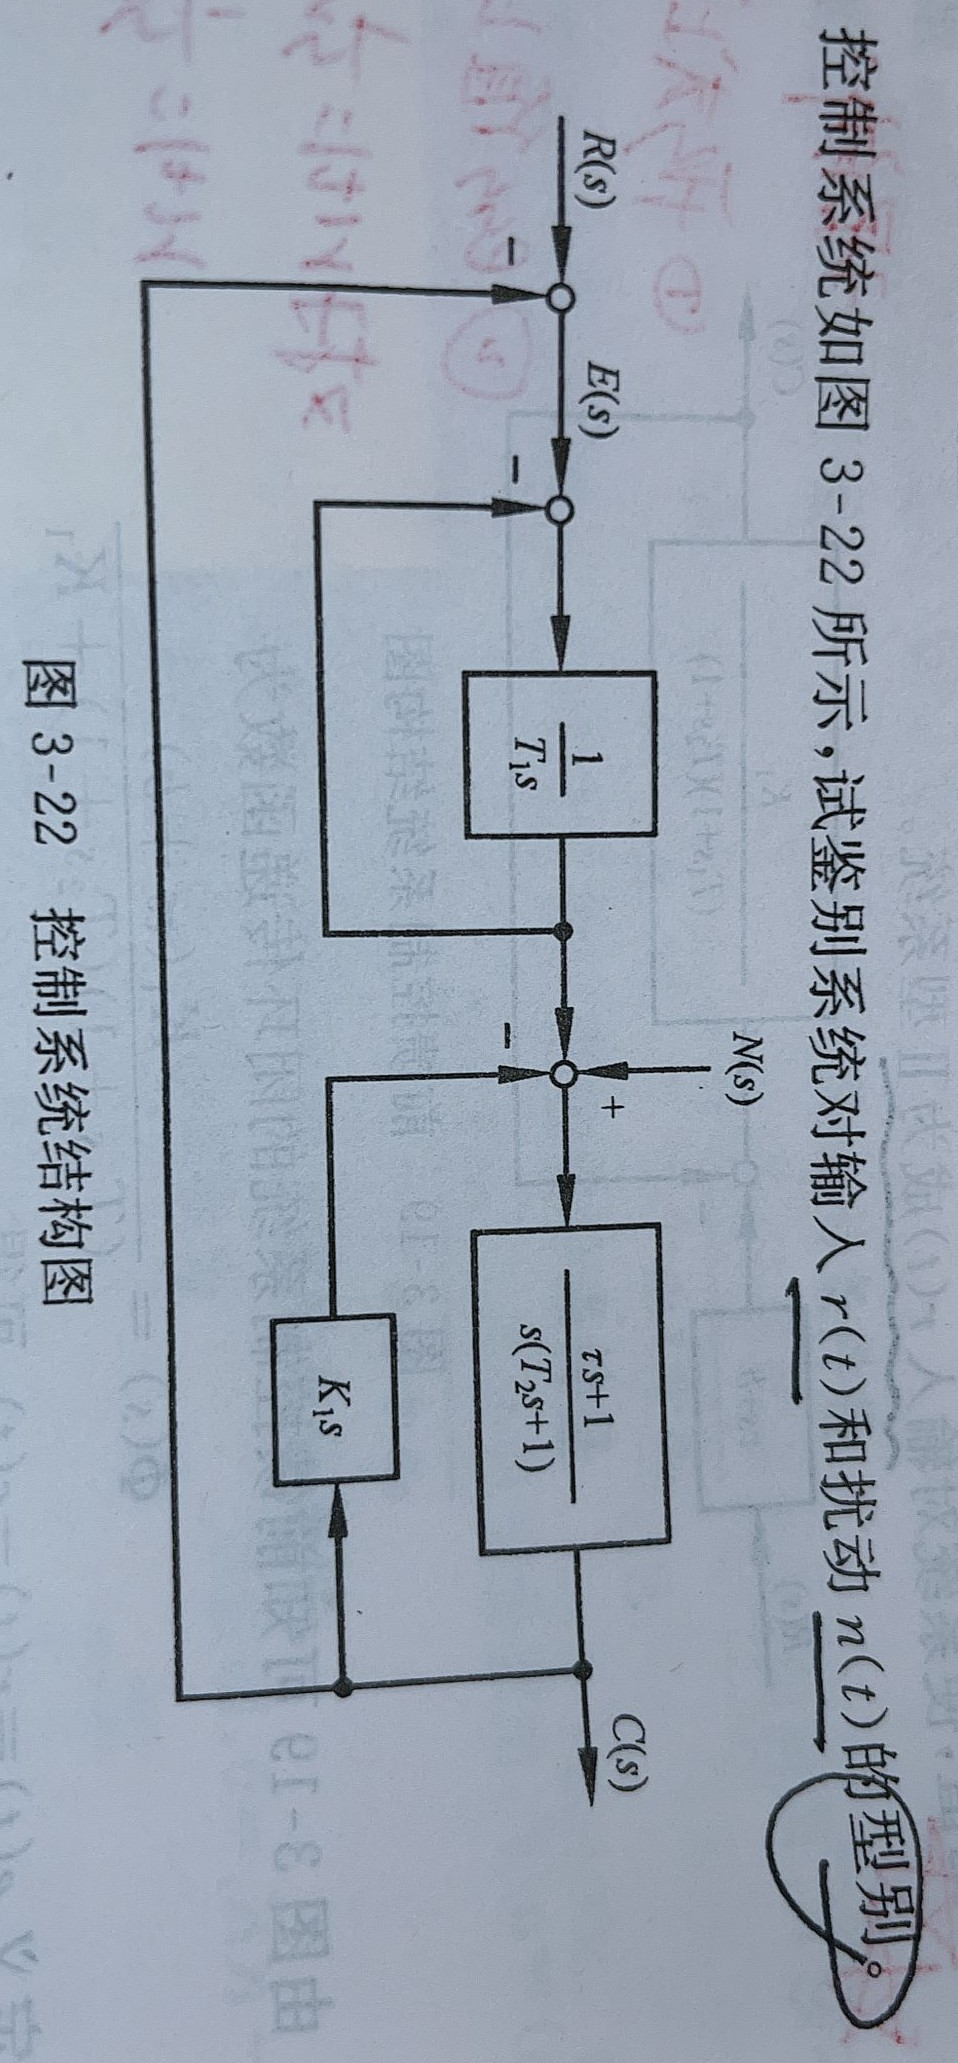
\includegraphics[height=0.9\textwidth, angle=90]{./pics/steady_state_error/example2.jpg}
    %最终文档中希望显示的图片标题
    \caption{例题2}
    %用于文内引用的标签
    \label{Fig.5}
\end{figure}

这道题明显可以分解,首先当$N(s)=0$时,很容易看出来,这是一个单位负反馈系统,
此时的$E(s)$也是输入端的定义,我们能够很容易的写出来$G(s)$。然后判断型别就好了。

但是当$R(s)=0$时,我们发现$E(s)$没有处于我们熟悉的定位位置,虽然我们可以通过一些
变换使得它变成输入端定义或者输出端定义,但是过多的操作无疑会增加我们的错误率。因此,
最好的办法就是写出$\frac{E(s)}{N(s)}$。

\end{document}
